\documentclass[a4paper,twoside,12pt]{article}
\usepackage[top=1.5cm,left=1.5cm,right=1.5cm,bottom=2cm]{geometry}

\usepackage[utf8]{inputenc}
\usepackage[T1]{fontenc}
\usepackage{lmodern}
\usepackage[brazilian]{babel}

\usepackage{graphicx}
\usepackage{subfig}
\usepackage{psfrag}
\usepackage{cite}
\usepackage[cmex10]{amsmath}
\usepackage{amssymb}
\usepackage{upgreek}
\usepackage{microtype}
\usepackage{titling}
\usepackage{courier}
\usepackage{url}
\usepackage{hyperref}
\hypersetup{
	colorlinks=true,
	linkcolor=blue,
	urlcolor=blue
}

% Use the 'listings' package to add code and the 'color' package to generate the highlights
\usepackage{listings}
\usepackage{color}
\definecolor{grey}{rgb}{0.6,0.6,0.6}
\definecolor{codegreen}{rgb}{0,0.6,0}
\definecolor{codegray}{rgb}{0.5,0.5,0.5}
\definecolor{codepurple}{rgb}{0.58,0,0.82}
\definecolor{backcolour}{rgb}{0.95,0.95,0.92}
\lstset{language=Python,				% set it to Python language highlighting
	backgroundcolor=\color{backcolour},
	commentstyle=\color{codegreen},
	keywordstyle=\color{magenta},
	numberstyle=\tiny\color{codegray},
	stringstyle=\color{codepurple},
	basicstyle=\ttfamily\small,		% set size of fonts
	breaklines=true,				% set automatic line breaking
	linewidth=\textwidth,			% set size of code box
	showstringspaces=false}			% show spaces as underscores only inside strings

\title{\vspace{-2cm} Processamento Digital de Sinais e Aplicações em Acústica\\ Tutorial 04 - Quantização}
\author{\url{https://github.com/fchirono/Aulas_PDS_Acustica}}

\begin{document}
	\date{}
	\maketitle
	
	\section*{Objetivos do Tutorial}
	Ao final desta sessão, você será capaz de:
		\begin{itemize}
		\item Simular um quantizador \emph{Linear Pulse Code Modulation} (L-PCM) do tipo \textit{midtread};
		\item Analisar o erro de quantização no domínio do tempo e da frequência;
		\item Compreender o efeito do número de bits na qualidade da representação
		digital;
		\item Aplicar e avaliar a técnica de \textit{dithering}.
	\end{itemize}

	\begingroup
	\let\clearpage\relax
	\tableofcontents
	\endgroup
	
	
	% ============================================================
	\section{Introdução}
	
	A conversão de um sinal analógico (contínuo no tempo e na amplitude) para um sinal digital envolve duas etapas fundamentais: a \textbf{amostragem}, que discretiza o sinal no tempo, e a \textbf{quantização}, que discretiza a amplitude do sinal. Este tutorial foca na segunda etapa.
	
	\subsection{O Processo de Quantização}
	
	Em um conversor analógico-digital (\textit{Analog-to-Digital Converter}, ADC), um sinal de tempo discreto $x[n]$ é mapeado para um conjunto finito de amplitudes discretas, denominados \textbf{níveis de quantização}. Para um conversor de $N_\text{bits}$ bits, o número total de níveis disponíveis é $2^{N_\text{bits}}$. Em sistemas bipolares (sinais com componentes positiva e negativa), um bit é reservado para o sinal, resultando em $2^{N_\text{bits}-1}$ níveis por polaridade. Como exemplo, a Figura \ref{fig:simbolo_binario} mostra os símbolos binários e seus valores numéricos (normalizados) para um conversor analógico-digital bipolar de 3 bits, com o primeiro bit indicando o sinal.
	
	\begin{figure}[h]
		\centering
		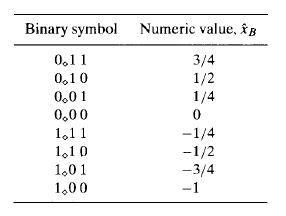
\includegraphics[width=0.4\textwidth]{SimboloBinario_ValorNumerico_OppenheimSchafer(2aEd).PNG}
		\caption{Tabela de símbolos binários e os valores numéricos normalizados para um ADC bipolar de 3 bits (Oppenheim e Schaefer, 1999).}
		\label{fig:simbolo_binario}
	\end{figure}
		
	Para um conversor bipolar com tensão elétrica máxima $V_\text{max}$ (isto é, que aceita tensões de entrada entre $-V_{max}$ e $+V_{max}$), o tamanho $\Delta v$ de cada nível de quantização (também chamado de ``bit menos significante'', ou \textit{Least Significant Bit} - LSB) é dado por:
	
	\begin{equation}
		\Delta v = \frac{2 \cdot V_\text{max}}{2^{N_\text{bits}-1}}.
		\label{eq:lsb}
	\end{equation}
	
	Para um conversor unipolar (que aceita tensões de entrada entre $0$ e $+V_{max}$), usa-se metade do valor dado pela Equação \ref{eq:lsb}.
	
	\subsection{Quantizador \textit{Midtread}}
	
	Neste tutorial utilizamos um quantizador do tipo \textit{midtread} (Lipshitz et al., 1992). O sinal quantizado $x_Q[n]$ é obtido através da expressão:
	
	\begin{equation}
		x_Q[n] = \Delta v \left\lfloor \frac{x[n]}{\Delta v} + \frac{1}{2}
		\right\rfloor
		\label{eq:midtread}
	\end{equation}
	
	\noindent onde $x[n]$ é o sinal discreto original e $\lfloor \cdot \rfloor$ denota a função piso (\textit{floor}).
	
	Caso o sinal de entrada apresente valores fora da faixa de tensão mínima e máxima do conversor, o conversor irá saturar e os valores convertidos são tipicamente ``ceifados'' (\emph{clipped}) - isto é, limitados aos valores mínimo e máximo de tensão do conversor. Para um conversor bipolar, isso pode ser descrito da forma:
	\begin{equation}
		x_Q[n] = 
		\begin{cases}
			+V_{max}, & \text{se } x[n] > +V_{max}, \\
			-V_{max}, & \text{se } x[n] < -V_{max}.
		\end{cases}
		\label{eq:clipping}
	\end{equation}
	
	Frequentemente o sinal quantizado é normalizado pela tensão máxima do quantizador, de forma que um sinal de máxima amplitude $x[n] = \pm V_{max}$ resulta em um sinal quantizado $x_Q[n] = \pm 1$. Esta normalização não será necessária neste Tutorial.
	
	\subsection{Erro de Quantização}
	
	Ao quantizar um sinal, inevitavelmente introduz-se um \textbf{erro de quantização} $e[n]$, definido como a diferença entre o sinal original e o sinal quantizado:
	\begin{equation}
		e[n] = x[n] - x_Q[n]
		\label{eq:erro}
	\end{equation}
	
	Para um sinal de entrada suficientemente complexo, o erro de quantização comporta-se aproximadamente como ruído branco com distribuição uniforme no intervalo $[-\Delta v/2,\, \Delta v/2]$. Nesse caso, a densidade espectral de potência do erro é aproximadamente plana, com valor teórico:
	\begin{equation}
		S_e(f) = \frac{\Delta v^2}{6\,f_s}
		\label{eq:psd_erro}
	\end{equation}
	onde $f_s$ é a frequência de amostragem.
	
	\subsection{\textit{Dithering}}
	
	Para sinais de magnitude comparável ao LSB, a quantização pode resultar em distorção harmônica audível e modulação de ruído indesejadas. Uma técnica eficaz para mitigar esse problema é o \textit{dithering}, que consiste em adicionar um ruído de baixa amplitude ao sinal antes da quantização, de forma a descorrelacionar o erro de quantização do sinal de entrada. Conforme descrito por Lipshitz et al.\ (1992):
	
	\begin{quote}
		\textit{``O objetivo do dithering é controlar as propriedades estatísticas do erro total e a sua relação com o sinal de entrada do sistema. Em sistemas sem dithering, sabemos que o erro é uma função determinística da entrada. Se o sinal de entrada for uma função simples ou com magnitude comparável ao nível de quantização, o sinal de erro total é fortemente dependente da entrada e será percebido como distorção grosseira e modulação de ruído. Veremos que o uso do dither com as propriedades estatísticas corretas pode tornar o erro total do sinal equivalente auditivamente a ruído branco constante.''}
	\end{quote}
	
	Como exemplo, o \textit{dithering} de espectro triangular pode ser obtido pela soma de dois sinais de ruído aleatório independentes com distribuição uniforme, cada um com amplitude $2 \cdot \Delta v$ pico a pico, e dividindo o sinal resultante por 2. O sinal de \textit{dither} é somado ao sinal original \textit{antes} da quantização.

	
	% ============================================================
	\section{Exercícios}
	
	% --------------------------------------------------
	\subsection{Função de Quantização}
	\label{sec:ex1}
	\begin{enumerate}
		\item Crie uma função em Python para calcular a versão quantizada de um sinal:
		\
\begin{lstlisting}[frame=single]
def quantizar_sinal(sinal, n_bits, v_max):

  [...]
	
  return sinal_quantizado, erro_quantizacao, tamanho_nivel
\end{lstlisting} 
		A função recebe como parâmetros de entrada um vetor de amostras do sinal ``analógico'', o número de bits utilizado no conversor, e a tensão máxima de entrada do conversor. A função deve retornar o vetor de amostras do sinal quantizado, o vetor de amostras do sinal de erro, e o tamanho do nível de quantização em Volts. A sua função deve implementar as Equações \ref{eq:lsb}-\ref{eq:erro}. Assuma um conversor com entrada bipolar (isto é, que aceita tensões de entrada entre $-V_{max}$ e $+V_{max}$). 
		
		\item Crie um sinal senoidal com os seguintes parâmetros:
		\begin{center}
			\begin{tabular}{ll}
				\textbf{Parâmetro} & \textbf{Valor} \\
				\hline
				Frequência de amostragem ($f_s$) & $44100$ Hz \\
				Duração do sinal ($T$)           & $2,0$ s \\
				Frequência da senoide ($f_0$)    & $123,4$ Hz \\
				Amplitude do sinal               & $1,25$ V$_{pico}$ \\
			\end{tabular}
		\end{center}
		
		Calcule o sinal quantizado por um conversor com $V_{max}=5$ Volts e $N_{bits}=4$ bits usando a função {\tt quantizar\_sinal}. Crie uma figura mostrando os primeiros 10 ms do sinal original, do sinal quantizado (no mesmo gráfico), e o sinal de erro (em um gráfico separado). Que características você observa no sinal de erro?
		% O sinal de erro apresenta padrão regular, indicando correlação entre o sinal de entrada e o sinal de erro.
		
		\item A densidade espectral de potência $S_{xx}(f)$ (tópico coberto em mais detalhes em tutoriais futuros) estima como a potência do sinal está distribuída no domínio da frequência. Esta função pode ser calculada e plotada da seguinte forma:
		
\begin{lstlisting}[frame=single]
# numero de pontos entre f=0 e f=fs
Ndft = 1024

# f: frequencias [Hz] / Sxx: densidade espectral de potencia [V^2/Hz]
f, Sxx = ss.welch(sinal, fs, 'hann', nperseg=Ndft,
        noverlap=Ndft//2, scaling='density')

# plotar Sxx com escala vertical logaritmica
plt.figure()
plt.semilogy(f, Sxx)
\end{lstlisting} 
		Calcule e plote a densidade espectral de potência do sinal original, do sinal quantizado, e do sinal de erro. O espectro do sinal quantizado é uma boa aproximação do espectro do sinal original? Como o espectro do sinal de erro está distribuído na frequência?
		
		\item Calcule a densidade espectral teórica do sinal de erro (dada pela Equação \ref{eq:psd_erro}) e trace uma linha horizontal no gráfico correspondente a esse valor. O valor teórico é uma boa aproximação da densidade espectral calculada?
	
		\item Auralize os sinais originais, quantizados, e de erro usando a função {\tt sounddevice.play}*. O sinal quantizado é uma boa aproximação do sinal original? Que características podem ser ouvidas no sinal quantizado?\\
		*\emph{CUIDADO COM O VOLUME DA AURALIZAÇÃO!}
		
		\item Repita o exercício usando $N_{bits}=8$ e $N_{bits}=16$. Qual é o impacto do aumento do número de bits do conversor?
	
	\end{enumerate}

	% --------------------------------------------------
	\subsection{Amplitude do Sinal e Saturação}
	\label{sec:ex2}
	
	Utilizando $N = 4$ bits e $f_0 = 123{,}4$ Hz, modifique a amplitude do sinal senoidal conforme indicado abaixo.
	
	\begin{enumerate}
		\item Aumente a amplitude de pico do sinal para 10 V. Inspecione o sinal quantizado e o erro.\\
		*\emph{CUIDADO COM O VOLUME DA AURALIZAÇÃO!}
		% Vpk > V_max, saturacao do conversor e distorcao da senoide.
		
		\item Reduza a amplitude de pico do sinal para 0.5 Volts. O que acontece com o sinal quantizado? O sinal é representado corretamente?
		% Vpk < Vlsb, o sinal nao é convertido
	\end{enumerate}
	
	
	% --------------------------------------------------
	\subsection{\textit{Dithering} (OPCIONAL)}
	\label{sec:ex3}
	
	Modifique a sua função {\tt quantizar\_sinal} para receber um parâmetro adicional de entrada {\tt dither}, que permite a aplicação de \emph{dither} ao sinal de entrada:
	
\begin{lstlisting}[frame=single]
def quantizar_sinal(sinal, n_bits, v_max, dither=False):

  if dither:
    [...]
	
  [...]
		
  return sinal_quantizado, erro_quantizacao, tamanho_nivel
\end{lstlisting} 
	
	
	\begin{enumerate}
		\item Implemente a aplicação opcional de dithering ao sinal de entrada na função {\tt quantizar\_sinal}.
		
		\item Compare o sinal de erro no domínio do tempo com e sem \textit{dithering}. O padrão determinístico é eliminado?
		
		\item Compare os espectros do erro com e sem \textit{dithering}. Os picos harmônicos são reduzidos? O nível de piso do erro aumenta ou diminui?
		
		\item \textbf{Auralização:} ouça os sinais com e sem \textit{dithering} para $N = 4$ bits. A distorção harmônica é reduzida com o \textit{dithering}? O ruído de fundo aumenta?
	\end{enumerate}
	
	
	% ============================================================
	\section{Referências}
	
	\begin{enumerate}
		\item A.~V.~Oppenheim e R.~W.~Schafer, \textit{Discrete-Time Signal
			Processing}, 2ª ed. Prentice-Hall, 1999. Seção 4.8.2.
		
		\item S.~P.~Lipshitz, R.~A.~Wannamaker e J.~Vanderkooy,
		``Quantization and Dither: A Theoretical Survey'', \textit{J.\
			Audio Eng.\ Soc.}, vol.~40, no.~5, pp.~355--375, 1992.
		\url{https://www.researchgate.net/publication/236340550}
	\end{enumerate}

\end{document}